\documentclass[tikz]{standalone}
\usetikzlibrary{spy,shapes,shadows,calc,pgfplots.groupplots}
\usepackage{amsmath}
\usepackage{physics} 
\usepackage{pgfplots}
\pgfplotsset{compat=1.3}
\usepackage{amsmath}
\usepackage{tcolorbox}
\DeclareFontFamily{OT1}{pzc}{}
\DeclareFontShape{OT1}{pzc}{m}{it}{<-> s * [1.10] pzcmi7t}{}
\DeclareMathAlphabet{\mathpzc}{OT1}{pzc}{m}{it}
\newcommand{\ddtn}{\operatorname{dtn}}

\pgfplotsset{
  %legend style = {font=\small}
}

%
\begin{document}
\begin{tikzpicture}[scale = 0.8, spy using outlines=
	{rectangle, 
	width=5cm,
        height=1cm,
	magnification=3.0, 
	connect spies}]

\begin{scope}

\draw[thick,->,black] (0.0, 0.25 ) -- (0.0, 3.5 );
%\draw[thick,->,black] (0.0, 0.25 ) -- (2.0, -1.4 );
%\draw[thick,->,black] (1.15, -1.5 ) -- (1.55, -2.05 );

\draw[] ( 0.0, 3.75  )  node[rotate=0 ]{   \Large  $ t$ };
%\draw[] ( 1.7, - 1.2  )  node[rotate=10 ]{   $ x_1 $ };
%\draw[] ( 1.8, - 2.0  )  node[rotate=0 ]{   $ x_2 $ };

\node (mode) at (2.0,1.75) {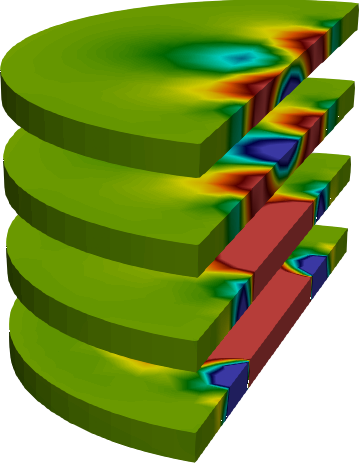
\includegraphics[scale =.2]{mode-cropped.png}};
\draw[] (2.0,4.25) node[draw, fill=white, minimum size=0.5mm]{ $\underline{u}_1^{\lambda}$ };
\end{scope}

\begin{scope}[xshift=5cm]
\begin{groupplot}[
    group style={
        %group name=dtn,
        group size=1 by 1,
        %xticklabels at=edge bottom,
        horizontal sep=25pt,
        vertical sep=40pt,
   },
   %name = dtnplot,
   height = 6.5cm,
   width = 8.5cm,
   every axis plot/.append style={thick},
   axis y line*=left,
   legend pos = south east,
    legend style = { column sep = 10pt, legend columns = 1, legend to name = grouplegend,},
   ]

    \nextgroupplot[ 
    ymode=log,
    xlabel= { \tcbox[size=fbox]{ $t$ }},
    %legend pos = south west,
    x label style={at={(axis description cs:0.95,0.075)},anchor=east},
    every axis title/.style={below right,at={(0.35,0.99)}},	
    title = {  \tcbox[size=fbox]{ $ \Vert \underline{u}_1^{\lambda}(t)  \Vert_{L^2 } $ } },
    legend style={at={(0.8,0.1)},anchor=north},
	]
   
    \addplot[green!70!black,very thick]  
	table[x=t,y=mass-omega] {../data/Cylinder-bad-mode-mass.dat} ;\addlegendentry{ $ \omega_T  $   } % 
    
    \addplot[red,very thick]  
        table[x=t,y=mass-B] {../data/Cylinder-bad-mode-mass.dat};  \addlegendentry{ $ B $  } %
    
    \addplot[cyan,very thick]  
	table[x=t,y=mass-complement] {../data/Cylinder-bad-mode-mass.dat};  \addlegendentry{ $ Q \setminus B  $  } %
     \end{groupplot}
    \node at ($(group c1r1) + (3.5cm,0.5cm)$) {\ref{grouplegend}};

\end{scope}

\begin{scope}[yshift=-6.5cm]
\begin{groupplot}[
    group style={
        %group name=dtn,
        group size=2 by 1,
        %xticklabels at=edge bottom,
        horizontal sep=25pt,
        vertical sep=40pt,
   },
   %name = dtnplot,
   height = 6.5cm,
   width = 8.5cm,
   every axis plot/.append style={thick},
   axis y line*=left,
   legend pos = south east,
   ]
    \nextgroupplot[ 
    ymode=log,
    xmode=log,
    %xmin=0,xmax=1.6e4,
    %xtick={25, 125, 250, 500, 800, 1000},
    %axis x line*=middle,
    %axis y line=middle, 
    %ymax = 1e-0,
    %xmin = 5e-2,
    ymax = 3.0e-1,
    ymin = 3e-2,
    %width=9cm,
    %restrict y to domain=-4e2:4e2,
    %xtick={0,2e3,4e3,6e3,8e3,10e3,12e3,14e3},
    xlabel= { $\sim h$},
    %legend pos = south west,
    x label style={at={(axis description cs:0.4,+0.075)},anchor=east},
	%title = {  $\norm{ u - \mathcal{L}_{\Delta t} \underline{u}_1 }_{L^2(Q)}$ },
    every axis title/.style={below right,at={(0.7,1.125)}},
	title = {   $ \theta = 1  $ },
    legend style={at={(0.8, 0.3)},anchor=north},
	]

    \addplot[blue,very thick,mark=*,forget plot,mark options={scale=0.1} ] 
   	table[x=deltat,y=L2-err-B] {../data/Cylinder-q1-qstar1-k1-kstar1-noise-smooth-theta1.dat};  
    \addplot[red,very thick,mark=o,forget plot,mark options={scale=0.1}  ]  
    	table[x=deltat,y=L2-err-B] {../data/Cylinder-q1-qstar1-k1-kstar1-noise-bad-mode-theta1.dat};  
   \addplot[lightgray] 
	table[mark=none,x=deltat,y expr ={1.54*\thisrowno{0} }] {../data/Cylinder-q1-qstar1-k1-kstar1-noise-smooth-theta1.dat};  \addlegendentry{$ \mathcal{O}(h) $ } %
    \addplot[black] 
	table[mark=none,x=deltat,y expr ={0.99*\thisrowno{0}^0.85}] {../data/Cylinder-q1-qstar1-k1-kstar1-noise-smooth-theta1.dat};  \addlegendentry{$ \mathcal{O}(h^{0.85}) $ } %
    \coordinate (spypoint) at (axis cs:0.026,0.04);
    \coordinate (magnifyglass) at (axis cs:0.035,0.125);
    \spy [black,width=3.0cm,height=1.75cm] on (spypoint) in node[fill=white] at (magnifyglass);
    
    \nextgroupplot[ 
    ymode=log,
    xmode=log,
    %xmin=0,xmax=1.6e4,
    %xtick={25, 125, 250, 500, 800, 1000},
    %axis x line*=middle,
    %axis y line=middle, 
    ymin = 5e-4,
    ymax = 8e-2,
    %xmin = 5e-2,
    %width=9cm,
    %restrict y to domain=-4e2:4e2,
    %xtick={0,2e3,4e3,6e3,8e3,10e3,12e3,14e3},
    xlabel= { $\sim h$},
    %legend pos = south west,
    %legend style = { column sep = 10pt, legend columns = 5, legend to name = grouplegend,},
    every axis title/.style={below right,at={(0.7,1.125)}},
    x label style={at={(axis description cs:0.4,+0.075)},anchor=east},
	%title = {  $\norm{ u - \mathcal{L}_{\Delta t} \underline{u}_1 }_{L^2(Q)}$ },
	title = { $  \theta = 2 $   },
    legend style={at={(0.8,0.5)},anchor=north},
	]

    \addplot[blue,very thick,mark=*,mark options={scale=0.1} ] 
	table[x=deltat,y=L2-err-B] {../data/Cylinder-q1-qstar1-k1-kstar1-noise-smooth-theta2.dat};  \addlegendentry{$ \delta u^{s} $ }  
    
    \addplot[red,very thick,mark=o,mark options={scale=0.1}  ]  
    	table[x=deltat,y=L2-err-B] {../data/Cylinder-q1-qstar1-k1-kstar1-noise-bad-mode-theta2.dat}; \addlegendentry{$ \delta u^{\lambda} $ }   
    
    \addplot[black] 
	table[mark=none,x=deltat,y expr ={0.925*\thisrowno{0}*\thisrowno{0}^0.7}] {../data/Cylinder-q1-qstar1-k1-kstar1-noise-smooth-theta2.dat};  \addlegendentry{$ \mathcal{O}(h^{1.7}) $ } %
    \addplot[lightgray] 
	table[mark=none,x=deltat,y expr ={1.625*\thisrowno{0}*\thisrowno{0}}] {../data/Cylinder-q1-qstar1-k1-kstar1-noise-smooth-theta2.dat};  \addlegendentry{$ \mathcal{O}(h^2) $ } %
 
    \coordinate (spypointB) at (axis cs:0.027,0.00125);
    \coordinate (magnifyglassB) at (axis cs:0.035,0.0125);
    \spy [black,width=3.0cm,height=2.45cm] on (spypointB) in node[fill=white] at (magnifyglassB);
    \end{groupplot}
\end{scope}


\end{tikzpicture}
\end{document}





